\documentclass[compress]{beamer}

\usetheme[block=fill]{metropolis}

\usepackage{graphicx} % Allows including images
\usepackage{amsmath,amsfonts,amsthm,amssymb}
\usepackage{color}
\usepackage{xcolor,cancel}
\usepackage{enumitem}
\setitemize{label=\usebeamerfont*{itemize item}%
	\usebeamercolor[fg]{itemize item}
	\usebeamertemplate{itemize item}}
\definecolor{mDarkBrown}{HTML}{604c38}
\definecolor{mDarkTeal}{HTML}{23373b}
\definecolor{mLightBrown}{HTML}{EB811B}
\definecolor{mMediumBrown}{HTML}{C87A2F}
\definecolor{mygreen}{HTML}{98C2B9}
\definecolor{myyellow}{HTML}{DFD79C}
\definecolor{myblue}{HTML}{8CA7CC}
\definecolor{kern}{HTML}{8CC2B7}


\usepackage{float}
\usepackage{framed}
\usepackage{epsfig}
\usepackage{graphicx}
\usepackage{subcaption}
\usepackage{ulem}
\usepackage{hhline}
\usepackage{multirow}
\usepackage{comment}   
\usepackage{bbm}
\usepackage{tikz}   
\def\Put(#1,#2)#3{\leavevmode\makebox(0,0){\put(#1,#2){#3}}}
\newcommand*\mystrut[1]{\vrule width0pt height0pt depth#1\relax}
\newcommand{\eqdef}{\mathbin{\stackrel{\rm def}{=}}}


\newcommand{\bs}[1]{\boldsymbol{#1}}
\newcommand{\bv}[1]{\mathbf{#1}}
\newcommand{\R}{\mathbb{R}}
\newcommand{\E}{\mathbb{E}}

\DeclareMathOperator*{\argmin}{arg\,min}
\DeclareMathOperator*{\argmax}{arg\,max}
\DeclareMathOperator{\nnz}{nnz}
\DeclareMathOperator{\diag}{diag}
\DeclareMathOperator{\Var}{Var}
\DeclareMathOperator{\sinc}{sinc}
\DeclareMathOperator{\sign}{sign}
\DeclareMathOperator{\dist}{dist}
\DeclareMathOperator{\mv}{mv}
\DeclareMathOperator{\sgn}{sgn}
\DeclareMathOperator{\step}{step}
\DeclareMathOperator{\gap}{gap}
\DeclareMathOperator{\poly}{poly}
\DeclareMathOperator{\tr}{tr}
\DeclareMathOperator{\orth}{orth}
\newcommand{\norm}[1]{\|#1\|}
\captionsetup[subfigure]{labelformat=empty}
\captionsetup[figure]{labelformat=empty}
\DeclareMathOperator*{\lmin}{\lambda_{min}}
\DeclareMathOperator*{\lmax}{\lambda_{max}}

\newcommand{\specialcell}[2][c]{%
  \begin{tabular}[#1]{@{}c@{}}#2\end{tabular}}
\newcommand{\specialcellleft}[2][c]{%
\begin{tabular}[#1]{@{}l@{}}#2\end{tabular}
}

\newtheorem{claim}[theorem]{Claim}
%\newtheorem{corollary}[theorem]{Corollary}

\usepackage{tabstackengine}
\stackMath


%----------------------------------------------------------------------------------------
%	TITLE PAGE
%----------------------------------------------------------------------------------------

\title{CS-GY 9223 D: Lecture 8 \\ Acceleration, preconditioning, coordinate methods}
\author{NYU Tandon School of Engineering, Prof. Christopher Musco}
\date{}

\begin{document}

\begin{frame}
	\titlepage 
\end{frame}

\metroset{titleformat=smallcaps}
\begin{frame}
	\frametitle{improving gradient descent}
	We now have a good understanding of gradient descent. 
	
	\textbf{Number of iterations for $\epsilon$ error:}
	\begin{center}
		\begin{tabular}{c|cc}
			& $G$-Lipschitz & $\beta$-smooth   \\ \hline
			$R$ bounded start & $O\left(\frac{G^2R^2}{\epsilon^2}\right)$ & $O\left(\frac{\beta R^2}{\epsilon}\right)$ \\
			$\alpha$-strong convex & $O\left(\frac{G^2}{\alpha\epsilon}\right)$ & $O\left(\frac{\beta}{\alpha}\log(1/\epsilon)\right)$
		\end{tabular}
	\end{center}
	
	\vspace{1em}
	\alert{How do we use this understanding to design \emph{faster algorithms?}}
\end{frame}

\begin{frame}[standout]
	\begin{center}
		\large acceleration
	\end{center}
\end{frame}


\begin{frame}
	\frametitle{accelerated gradient descent}
	\textbf{Nesterov's accelerated gradient descent}:
	\begin{itemize}
		\item $\bv{x}^{(1)} = \bv{y}^{(1)} = \bv{z}^{(1)}$  
		\item For $t = 1,\ldots, T$
		\begin{itemize}
			\item $\bv{y}^{(t+1)} = \bv{x}^{(t)} - \frac{1}{\beta}\nabla f(\bv{x}^{(t)})$
			\item $\bv{x}^{(t+1)} = \left(1 + \frac{\sqrt{\kappa} - 1}{\sqrt{\kappa} + 1}\right) \bv{y}^{(t+1)} + \frac{\sqrt{\kappa} - 1}{\sqrt{\kappa} + 1}\left(\bv{y}^{(t+1)} - \bv{y}^{(t)}\right)$
		\end{itemize}
	\end{itemize}
	\begin{theorem}[AGD for $\beta$-smooth, $\alpha$-strongly convex.]
		Let $f$ be a $\beta$-smooth and $\alpha$-strongly convex function. If we run AGD for $T$ steps we have:
		\begin{align*}
			f(\bv{x}^{(t)}) - f(\bv{x}^*) \leq \kappa e^{-(t-1)\sqrt{\kappa}} \left[f(\bv{x}^{(1)}) - f(\bv{x}^*) \right]
		\end{align*} 
	\end{theorem}	
	\textbf{Corollary:} If \alert{$T = O\left(\sqrt{\kappa}\log(\kappa/\epsilon)\right)$ achieve error $\epsilon$.} 
	
\end{frame}
%
%\begin{frame}[t]
%	\frametitle{linear regression runtime}
%	\textbf{Total runtime for solving linear regression via GD}:
%	\begin{center}
%		(time per iteration) x (number of iterations)
%		
%		\vspace{5em}
%		
%		\large
%		$\alert{O(nd\cdot\kappa\log(1/\epsilon))}$
%		
%		for $\bv{A}\in \R^{n\times d}$, $\bv{x} \in \R^d$, $\bv{b}\in \R^n$.
%	\end{center}	
%\end{frame}
%
%\begin{frame}[t]
%	\frametitle{acceleration}
%	\begin{theorem}[Accelerated Iterative Regression]
%		Let $\bv{x}^* = \min_{\bv{x}}\|\bv{A}\bv{x} - \bv{b}\|_2^2$. There is an algorithm which finds $\tilde{\bv{x}} $ with $\|\tilde{\bv{x}} - \bv{x}^*\|_2 \leq \epsilon\|\bv{x}^*\|_2$ in time:
%			\begin{align*}
%				O(nd\cdot\sqrt{\kappa\log(1/\epsilon)})
%			\end{align*} 
%	\end{theorem}
%\end{frame}
%
%\begin{frame}[t]
%	\frametitle{the polynomial view}
%	\textbf{Claim:} For any $\eta$, polynomial $p(z) = c_1 z + c_2 z^2 + \ldots + c_q z^q$ with $p(1) = \sum_{j=1}^q c_q = 1$, there is an algorithm running in $O(ndq)$ time which outputs $\tilde{\bv{x}}$ satisfying:
%	\begin{align*}
%	\tilde{\bv{x}} - \bv{x}^* =  p(\bv{I} - \frac{1}{\eta}\bv{A}^T\bv{A}) \bv{x}^*
%	\end{align*}
%	
%	\begin{center}
%		\alert{For standard gradient descent, $p(z) = z^q$.}
%	\end{center}
%\end{frame}
%
%\begin{frame}[t]
%	\frametitle{the polynomial view}
%	\textbf{Claim:} For any $\eta$, polynomial $p(z) = c_1 z + c_2 z^2 + \ldots + c_q z^q$ with $p(1) = \sum_{j=1}^q c_q = 1$, there is an algorithm running in $O(ndq)$ time which outputs $\tilde{\bv{x}}$ satisfying:
%	\begin{align*}
%	\tilde{\bv{x}} - \bv{x}^* =  c_1\cdot (\bv{I} - \eta\bv{A}^T\bv{A})\bv{x}^* + c_2 \cdot (\bv{I} - \eta\bv{A}^T\bv{A})^2  \bv{x}^* + \ldots + c_q \cdot (\bv{I} - \eta\bv{A}^T\bv{A})^q  \bv{x}^* 
%	\end{align*}
%	
%	\textbf{Claim:} $c_j  \cdot \bv{I} - \eta\bv{A}^T\bv{A})^j\bv{x}^* = c_j\cdot\bv{x}^* + p_j'(\bv{I} - \eta\bv{A}^T\bv{A})\bv{A}^T\bv{A}\bv{x}^*$ where $p_j$ is a polynomial with degree $j - 1$.
%\end{frame}
%
%\begin{frame}[t]
%	\frametitle{the polynomial view}
%	\textbf{Claim:} For any $\eta$, polynomial $p(z) = c_1 z + c_2 z^2 + \ldots + c_q z^q$ with $p(1) = \sum_{j=1}^q c_q = 1$, there is an algorithm running in $O(ndq)$ time which outputs $\tilde{\bv{x}}$ satisfying:
%	\begin{align*}
%	\bv{x}^* - \tilde{\bv{x}} &=  (c_1 + c_2 + \ldots + c_q)\cdot\bv{x}^* +  p'(\bv{I} - \eta\bv{A}^T\bv{A})\bv{A}^T\bv{A}\bv{x}^*
%	\end{align*}
%	\begin{align*}
%		\tilde{\bv{x}}  &= p'(\bv{I} - \eta\bv{A}^T\bv{A})\bv{A}^T\bv{b} \text{ where $p'$ is a polynmial with degree $q-1$}.
%	\end{align*}
%\end{frame}
%
%\begin{frame}[t]
%	\frametitle{the polynomial view}
%	\begin{align*}
%	\tilde{\bv{x}} - \bv{x}^* =  p(\bv{I} - \eta\bv{A}^T\bv{A})\bv{x}^*\\
%	p(\bv{I} - \eta\bv{A}^T\bv{A}) = \bv{U}p(\bv{I} - \eta\bs{\Lambda})\bv{U}^T
%	\end{align*}
%	
%	\begin{align*}
%	\|\tilde{\bv{x}} - \bv{x}^*\|  &= \|\bv{U}p(\bv{I} - \eta\bs{\Lambda})\bv{U}^T\bv{x}^*\|_2 \\
%	& = \|p(\bv{I} - \eta\bs{\Lambda})\bv{U}^T\bv{x}^*\|_2
%	\end{align*}
%	
%	As long as $\max\left[ p(\bv{I} - \eta\bs{\Lambda})\right] \leq \epsilon$, 
%	\begin{align*}
%	\|\tilde{\bv{x}} - \bv{x}^*\|_2  \leq \epsilon \|\bv{x}^*\|_2 
%	\end{align*}
%\end{frame}
%
%\begin{frame}[t]
%	\frametitle{constructing a jump polynomial}
%	\textbf{Goal:} Find polynomial $p$ such that $p(1) = 1$ and $p(z) \leq \epsilon$ for $z\in [0,1 - \frac{1}{\kappa}]$.
%	\begin{center}
%		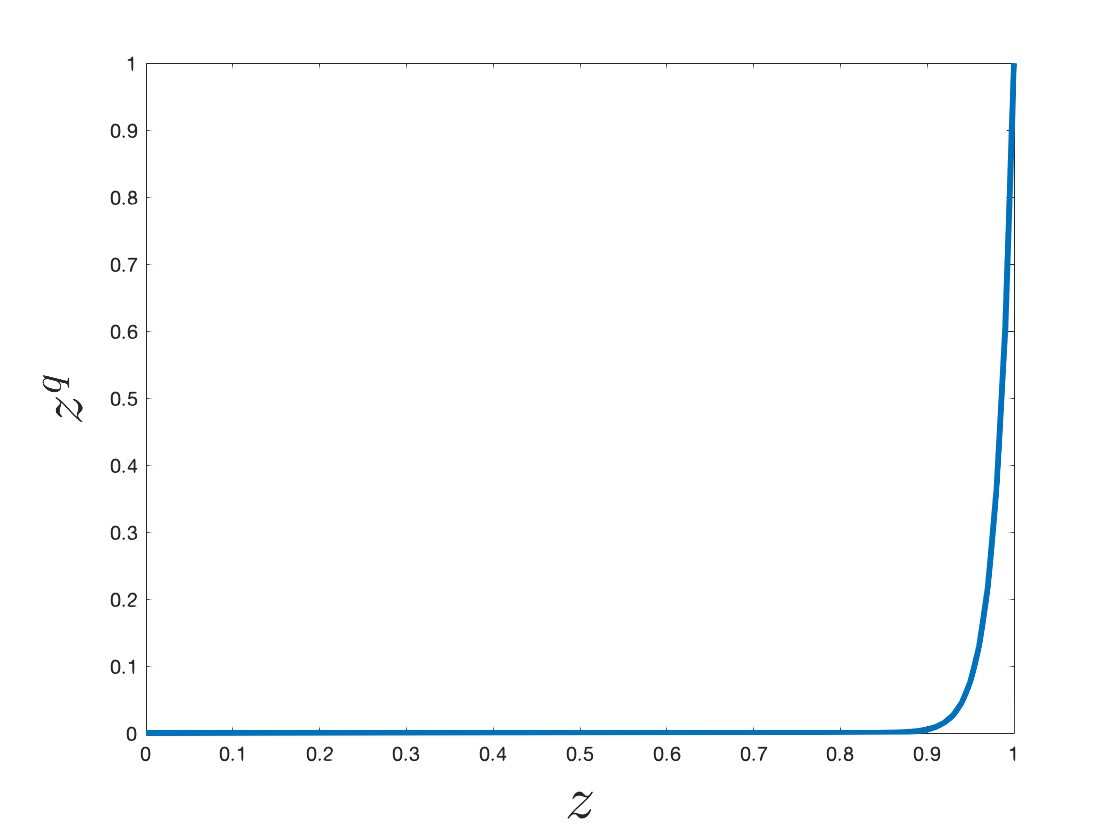
\includegraphics[width=.6\textwidth]{basic_jump.png}
%		
%		Gradient descent uses $p(z) = z^{O(\kappa\log(1/\epsilon))}$.
%	\end{center}
%\end{frame}
%
%\begin{frame}[t]
%	\frametitle{a better jump polynomial}
%		\textbf{Goal:} Find polynomial $p$ such that $p(1) = 1$ and $p(z) \leq \epsilon$ for $z\in [0,1 - \frac{1}{\kappa}]$.
%	\begin{center}
%		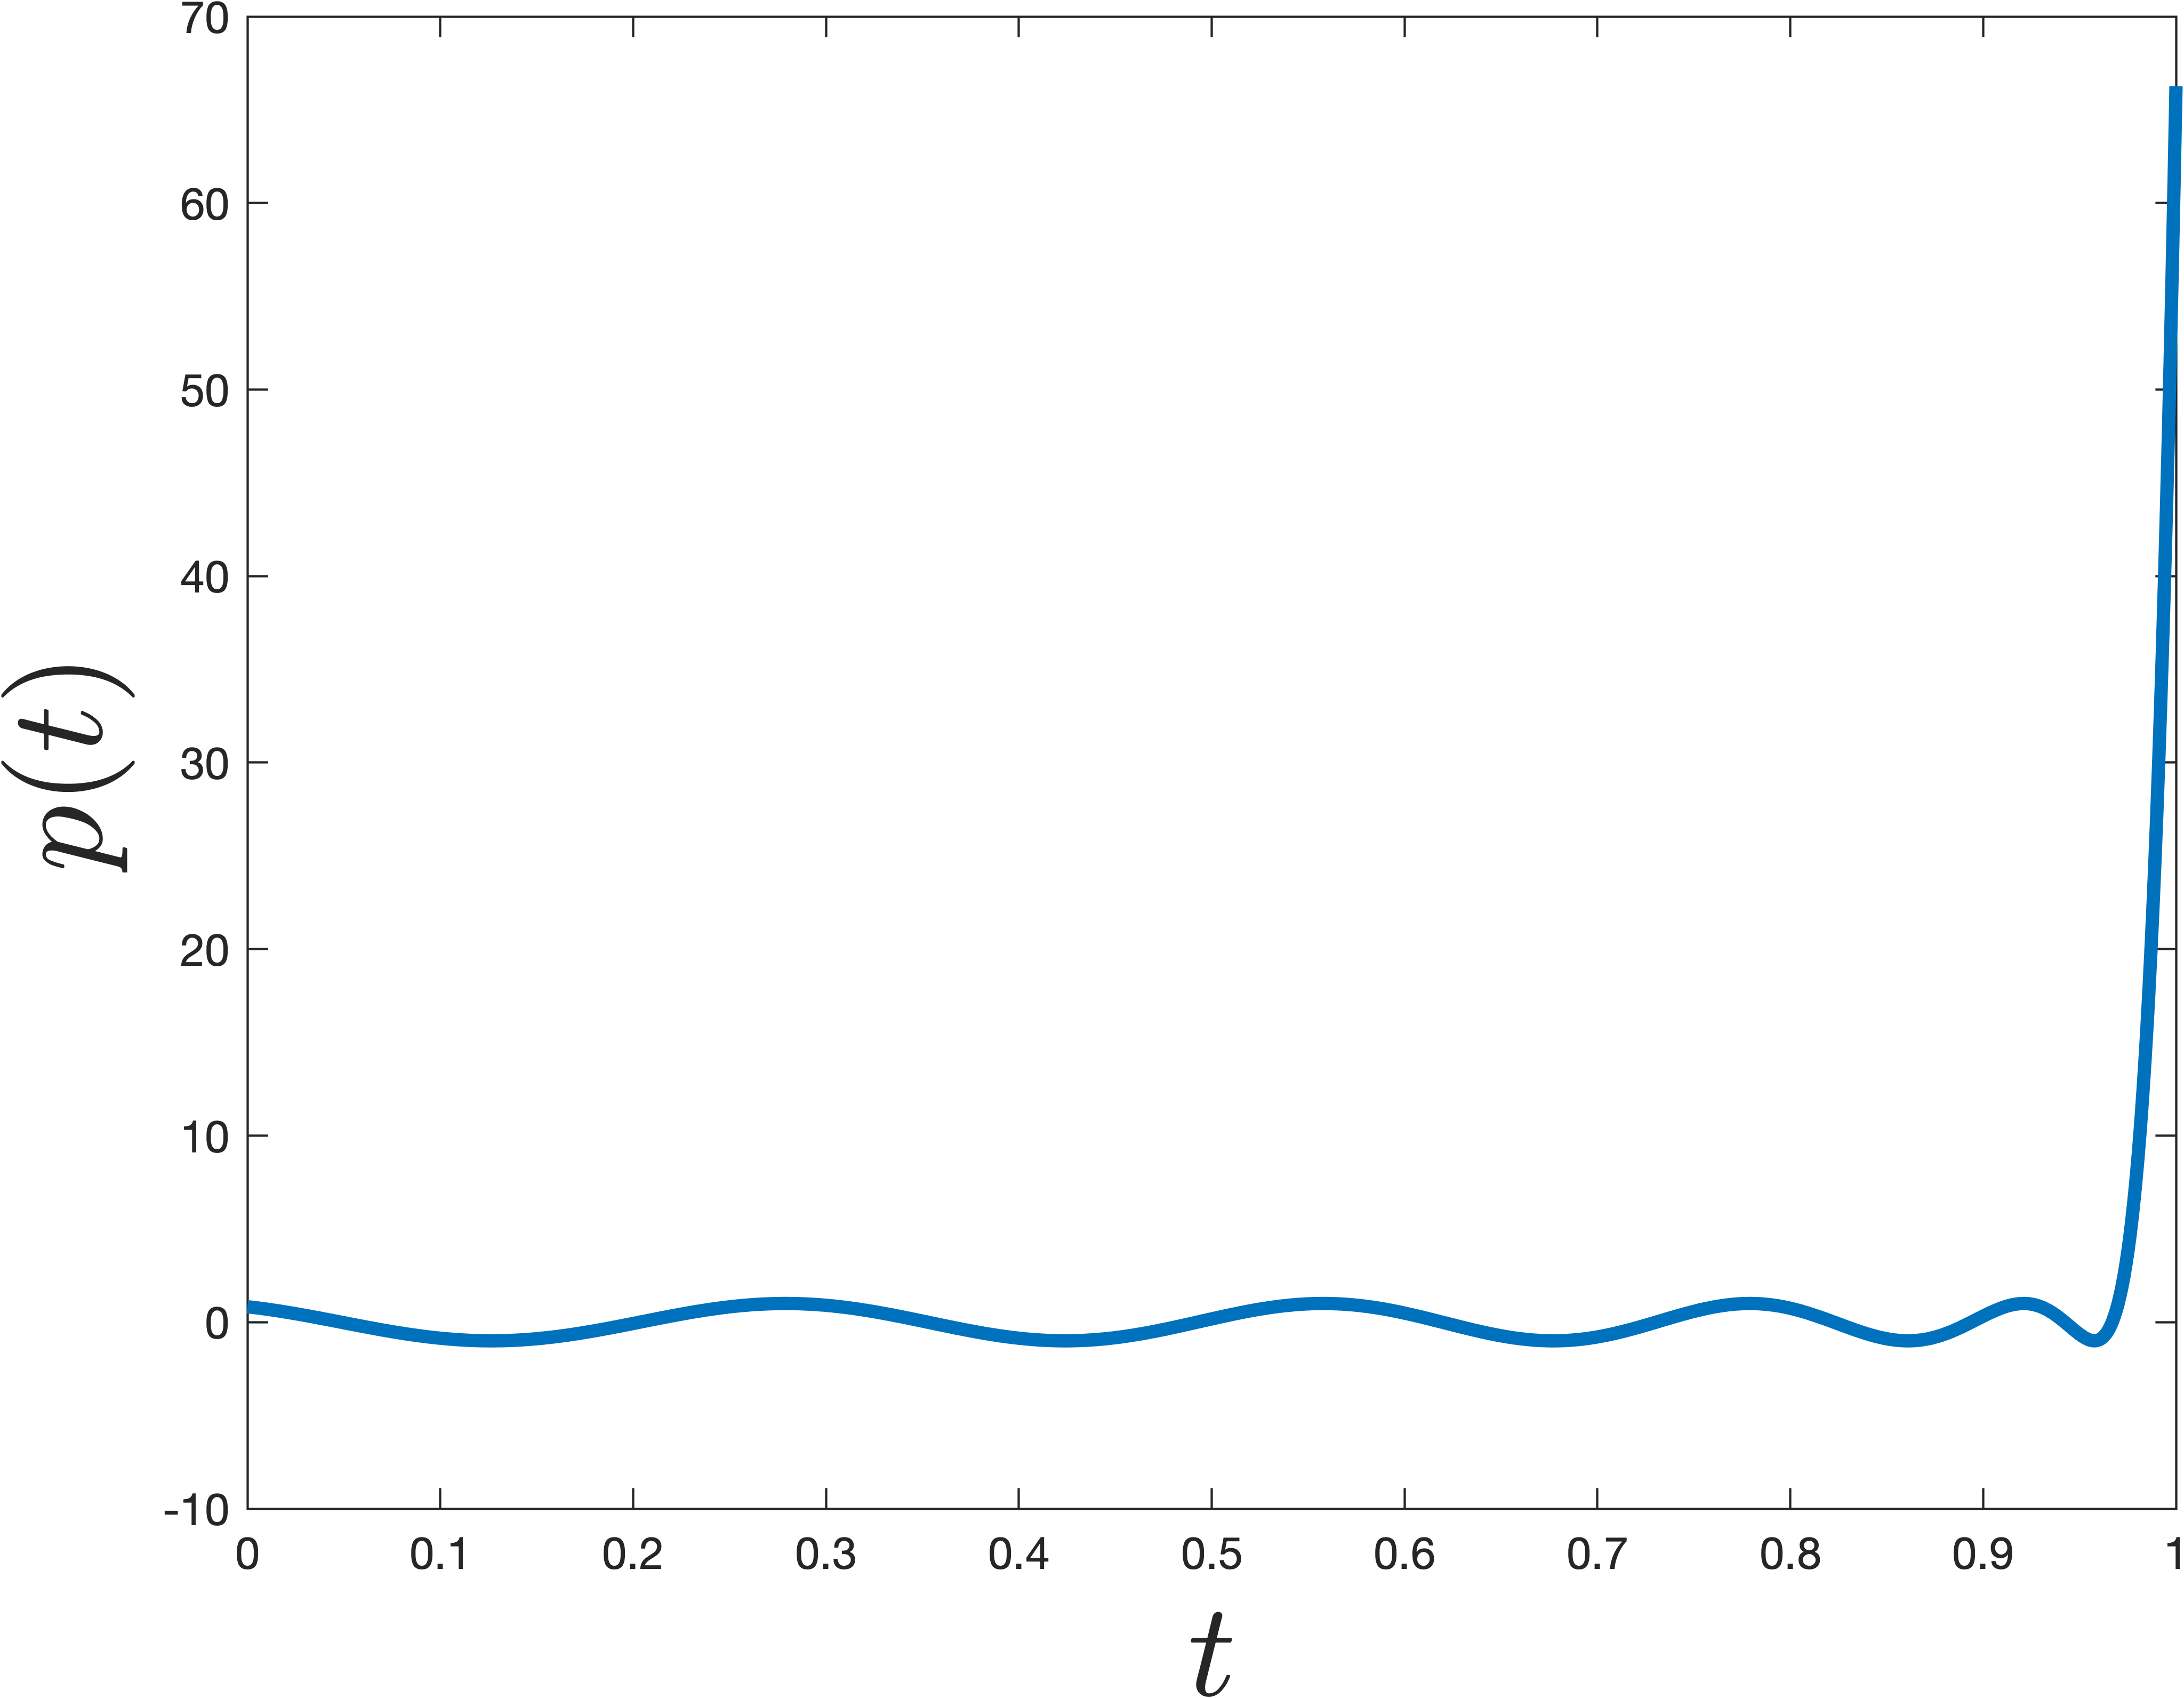
\includegraphics[width=.6\textwidth]{cheby_jump.png}
%		
%		\alert{Can be done with degree $O(\sqrt{\kappa\log(1/\epsilon)})$ polynomial instead!}
%	\end{center}
%\end{frame}
%
%\begin{frame}
%	\frametitle{chebyshev polynomials}
%	\begin{center}
%		\textbf{What are these polynomials?}
%	\end{center}
%	
%		\centering
%		Chebyshev polynomials of the first kind.
%		\begin{columns}
%			\begin{column}{0.5\textwidth}
%				\begin{align*}
%				T_0(x) &= 1\\
%				T_1(x) &= x \\
%				T_2(x) &= 2x^2 - 1\\
%				&\,\,\,\vdots\\
%				T_k(x) &= 2xT_{k-1}(x) - T_{k-2}(x)\\
%				\end{align*}
%			\end{column}
%			\begin{column}{0.5\textwidth}
%				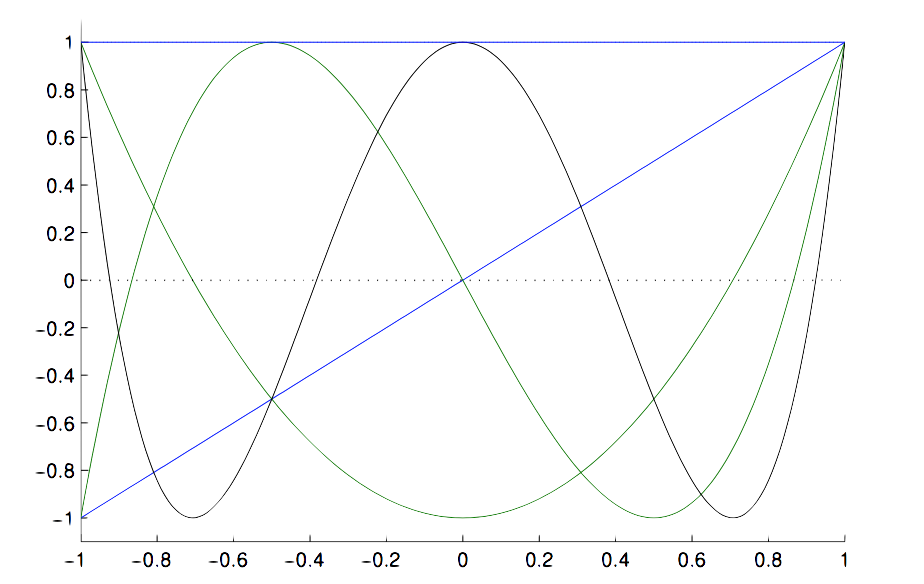
\includegraphics[width=\textwidth]{chebyPolys.png}
%			\end{column}
%		\end{columns}
%		\begin{center}
%			\textbf{``There's only one bullet in the gun. It's called the Chebyshev polynomial.''} -- Prof. Rocco Servedio
%		\end{center}
%\end{frame}
%
%\begin{frame}
%	\frametitle{accelerated gradient descent}
%	\textbf{Nesterov's accelerated gradient descent}:
%	\begin{itemize}
%		\item $\bv{x}^{(1)} = \bv{y}^{(1)} = \bv{z}^{(1)}$  
%		\item For $t = 1,\ldots, T$
%		\begin{itemize}
%			\item $\bv{y}^{(t+1)} = \bv{x}^{(t)} - \frac{1}{\beta}\nabla f(\bv{x}^{(t)})$
%			\item $\bv{x}^{(t+1)} = \left(1 + \frac{\sqrt{\kappa} - 1}{\sqrt{\kappa} + 1}\right) \bv{y}^{(t+1)} - \frac{\sqrt{\kappa} - 1}{\sqrt{\kappa} + 1}\bv{y}^{(t)}$
%		\end{itemize}
%	\end{itemize}
%	\begin{theorem}[AGD for $\beta$-smooth, $\alpha$-strongly convex.]
%	Let $f$ be a $\beta$-smooth and $\alpha$-strongly convex function. If we run AGD for $T$ steps we have:
%	\begin{align*}
%	f(\bv{x}^{(t)}) - f(\bv{x}^*) \leq \kappa e^{-(t-1)\sqrt{\kappa}} \left[f(\bv{x}^{(1)}) - f(\bv{x}^*) \right]
%	\end{align*} 
%\end{theorem}	
%\textbf{Corollary:} If \alert{$T = O\left(\sqrt{\kappa}\log(\kappa/\epsilon)\right)$ achieve error $\epsilon$.} 
%	
%\end{frame}

\begin{frame}[t]
	\frametitle{intuition behind acceleration}
	\begin{center}
		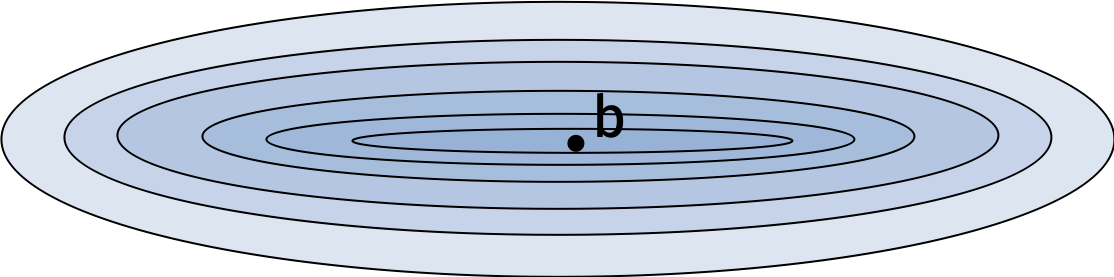
\includegraphics[width=\textwidth]{poor_conditioning.png}
		
		Level sets of $\|\bv{A}\bv{x} - \bv{b}\|_2^2$.
	\end{center}
	
	\textbf{Other terms for similar ideas:}
	\begin{itemize}
		\item Momentum
		\item Heavy-ball methods
	\end{itemize}
	
	\begin{center}
		\alert{What if we look back beyond \emph{two iterates}?}
	\end{center}
\end{frame}

\begin{frame}[standout]
	\begin{center}
		\large preconditioning
	\end{center}
\end{frame}

\begin{frame}
	\frametitle{preconditioning}
	\textbf{Main idea:}
	Instead of minimizing $f(\bv{x})$, find another function $g(\bv{x})$ with the same minimum but which is better suited for first order optimization (e.g., has a smaller conditioner number).
	
	\vspace{2em}
	\textbf{Claim:} Let $h(\bv{x}): \R^d \rightarrow \R^d$ be an \emph{invertible function}. Let $g(\bv{x}) = f(h(\bv{x}))$. Then
	\begin{align*}
		\alert{\min_{\bv{x}} f(\bv{x})} &\alert{= \min_{\bv{x}} g(\bv{x})} & &\text{and} & \alert{\argmin_{\bv{x}} f(\bv{x})} &\alert{= h\left(\argmin_{\bv{x}} g(\bv{x})\right)}.
	\end{align*}
\end{frame}

\begin{frame}[t]
	\frametitle{preconditioning}
	\textbf{First Goal:} We need $g(\bv{x})$ to still be convex.
	
	\textbf{Claim:} Let $\bv{P}$ be an (invertible) $d\times d$ matrix and let $g(\bv{x}) = f(\bv{P}\bv{x})$. 
	\begin{center} 
		\alert{$g(\bv{x})$ is always convex.}
	\end{center}

\vspace{10em}
If $\bv{y}^* = \argmin g(\bv{y})$, then $\bv{x}^* = \bv{P}\bv{y}^*$ minimizes $f(\bv{x})$. 
\end{frame}

\begin{frame}[t]
	\frametitle{preconditioning}
	\textbf{Second Goal:} 
	
	$g(\bv{x})$ should have better condition number $\kappa$ than $f(\bv{x})$. 
	
	
	\textbf{High dimensional chain rule:}
	\begin{align*}
		\text{If } g(\bv{x}) &= f(\bv{Px}), & \nabla^2 g(\bv{x}) = \nabla^2 \bv{P}^Tf(\bv{P}\bv{x})\bv{P}.
	\end{align*}
	Recall that the condition number is equal to:
	\begin{align*}
		\max_\bv{x} \frac{\lmax\left(\nabla^2 g(\bv{x})\right)}{\lmin\left(\nabla^2 g(\bv{x})\right)}
	\end{align*}
\end{frame}

\begin{frame}[t]
	\frametitle{preconditioning}
	\textbf{Example:} 
	\begin{itemize}
		\item $f(\bv{x}) = \|\bv{A}\bv{x} - \bv{b}\|_2^2$. $\nabla f(\bv{x}) = 2\bv{A}^T\bv{A}$. $\kappa_f =\frac{\lambda_1(\bv{A}^T\bv{A})}{\lambda_d(\bv{A}^T\bv{A})}$.
		\item $g(\bv{x}) = \|\bv{A}\bv{P}\bv{x} - \bv{b}\|_2^2$. $\nabla g(\bv{x}) = 2\bv{P}^T\bv{A}^T\bv{A}\bv{P}$ $\kappa_g =\frac{\lambda_1(\bv{P}^T\bv{A}^T\bv{A}\bv{P})}{\lambda_d(\bv{P}^T\bv{A}^T\bv{A}\bv{P})}$.
	\end{itemize}
	
	\textbf{Ideal preconditioner:} Choose $P$ so that  $\bv{P}^T\bv{A}^T\bv{A}\bv{P} = \bv{I}$. For example, could set $P = \sqrt{(\bv{A}^T\bv{A})^{-1}}$. But obviously this is too expensive to compute.
\end{frame}

\begin{frame}[t]
	\frametitle{diagonal preconditioner}
	\textbf{Third Goal:} $\bv{P}$ should be easy to compute.
	
	\begin{center}
		\alert{Many, many problem specific preconditioners are used in practice. There design is usually a heuristic process.} 
	\end{center}
	
	\textbf{Example:} Diagonal preconditioner for least squares problems. 
	\begin{itemize}
		\item Let $\bv{D} = \diag(\bv{A}^T\bv{A})$
		\item Want $\bv{PA}^T\bv{AP}$ to be close to identity $\bv{I}$.
		\item Let $\bv{P} = \sqrt{\bv{D}^{-1}}$
	\end{itemize}
	$\bv{P}$ is often called a \alert{\textbf{Jacobi preconditioner}}. Often works very well in practice!
\end{frame}

\begin{frame}
	\frametitle{diagonal preconditioner}
	\begin{center}
		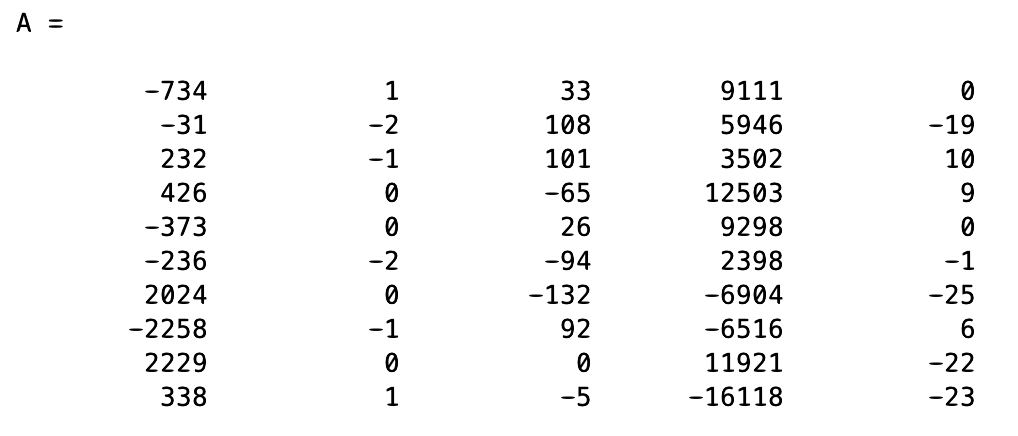
\includegraphics[width=.7\textwidth]{poorly_cond_a.png}
	\end{center}
	\vspace{2em}
	
	\begin{columns}[t]
		\begin{column}{0.3\textwidth}
			\vspace{-6.4em}
			
			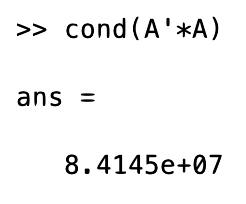
\includegraphics[width=.8\textwidth]{cond1.png}
		\end{column}
		\begin{column}{0.7\textwidth}
			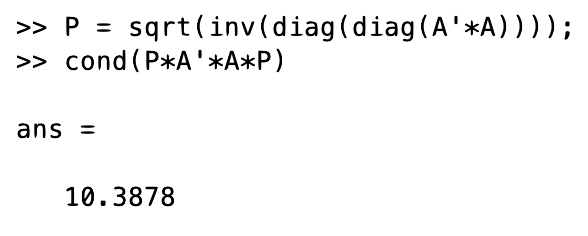
\includegraphics[width=.8\textwidth]{cond2.png}
		\end{column}
	\end{columns}
\end{frame}

\begin{frame}
	\frametitle{diagonal preconditioner intuition}
	$g(\bv{x}) = f(\|\bv{A}\bv{P}\bv{x} - \bv{b}\|_2^2)$ is the same least squares problem as $f(\bv{x}) = \|\bv{A}\bv{x} - \bv{b}\|_2^2$, but with each feature (column of $\bv{A}$) scaled differently. The $i^\text{th}$ column is scaled by $P_{ii}$. 
	\begin{center}
	\vspace{-.5em}
	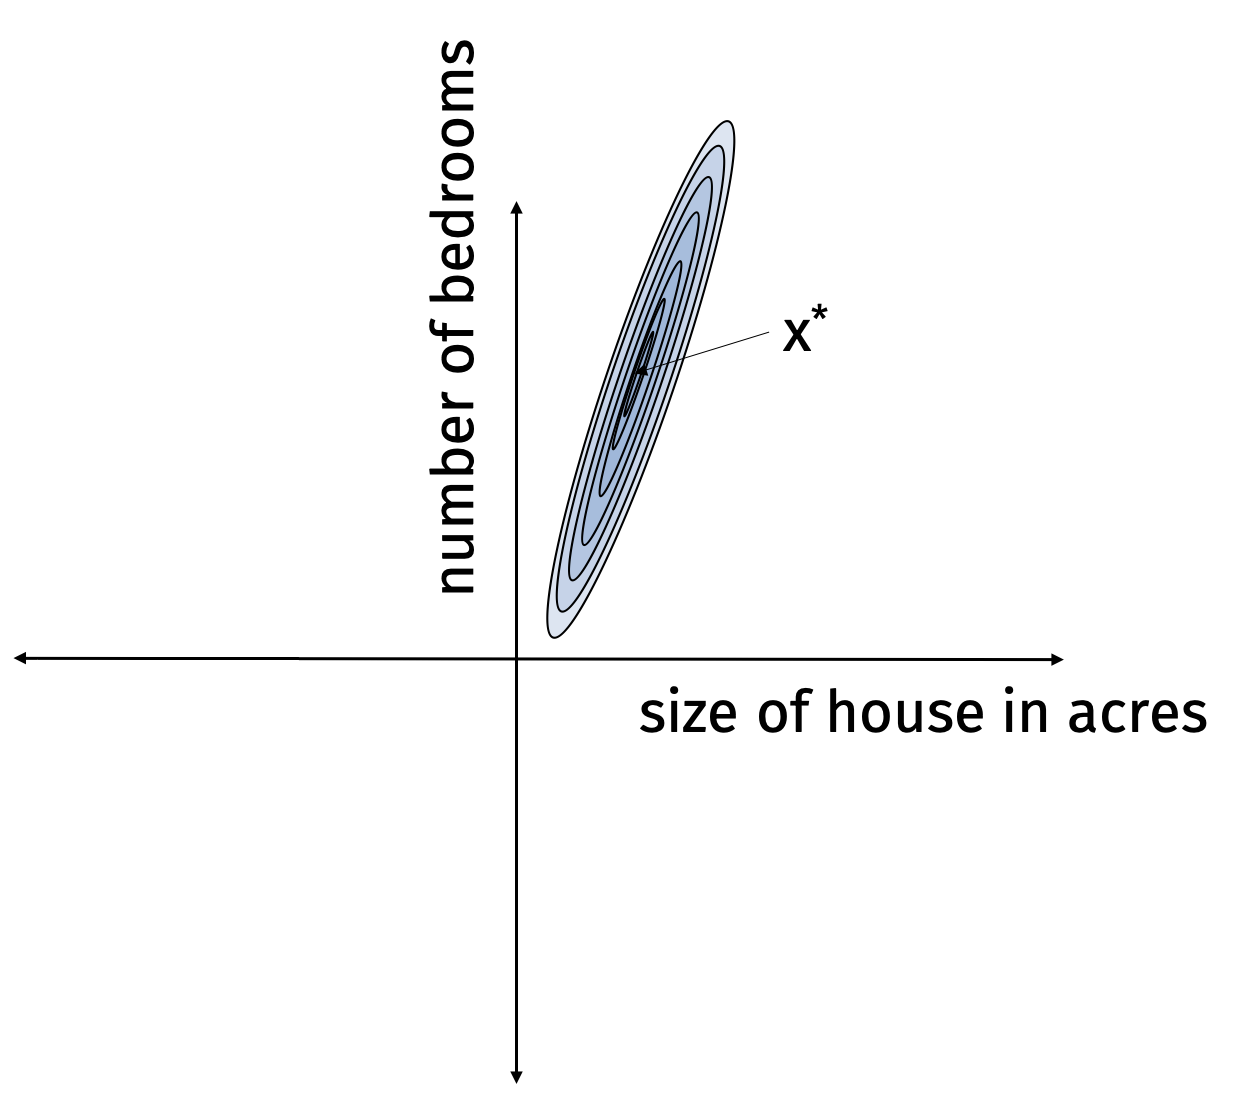
\includegraphics[width=.6\textwidth]{bad_scaling.png}
	\vspace{-.5em}
	
	Feature scaling can have a huge impact on conditioning. 
	\end{center}
\end{frame}

\begin{frame}
	\frametitle{diagonal preconditioner intuition}
	$g(\bv{x}) = f(\|\bv{A}\bv{P}\bv{x} - \bv{b}\|_2^2)$ is the same least squares problem as $f(\bv{x}) = \|\bv{A}\bv{x} - \bv{b}\|_2^2$, but with each feature (column of $\bv{A}$) scaled differently. The $i^\text{th}$ column is scaled by $P_{ii}$. 
	\begin{center}
		\vspace{-.5em}
		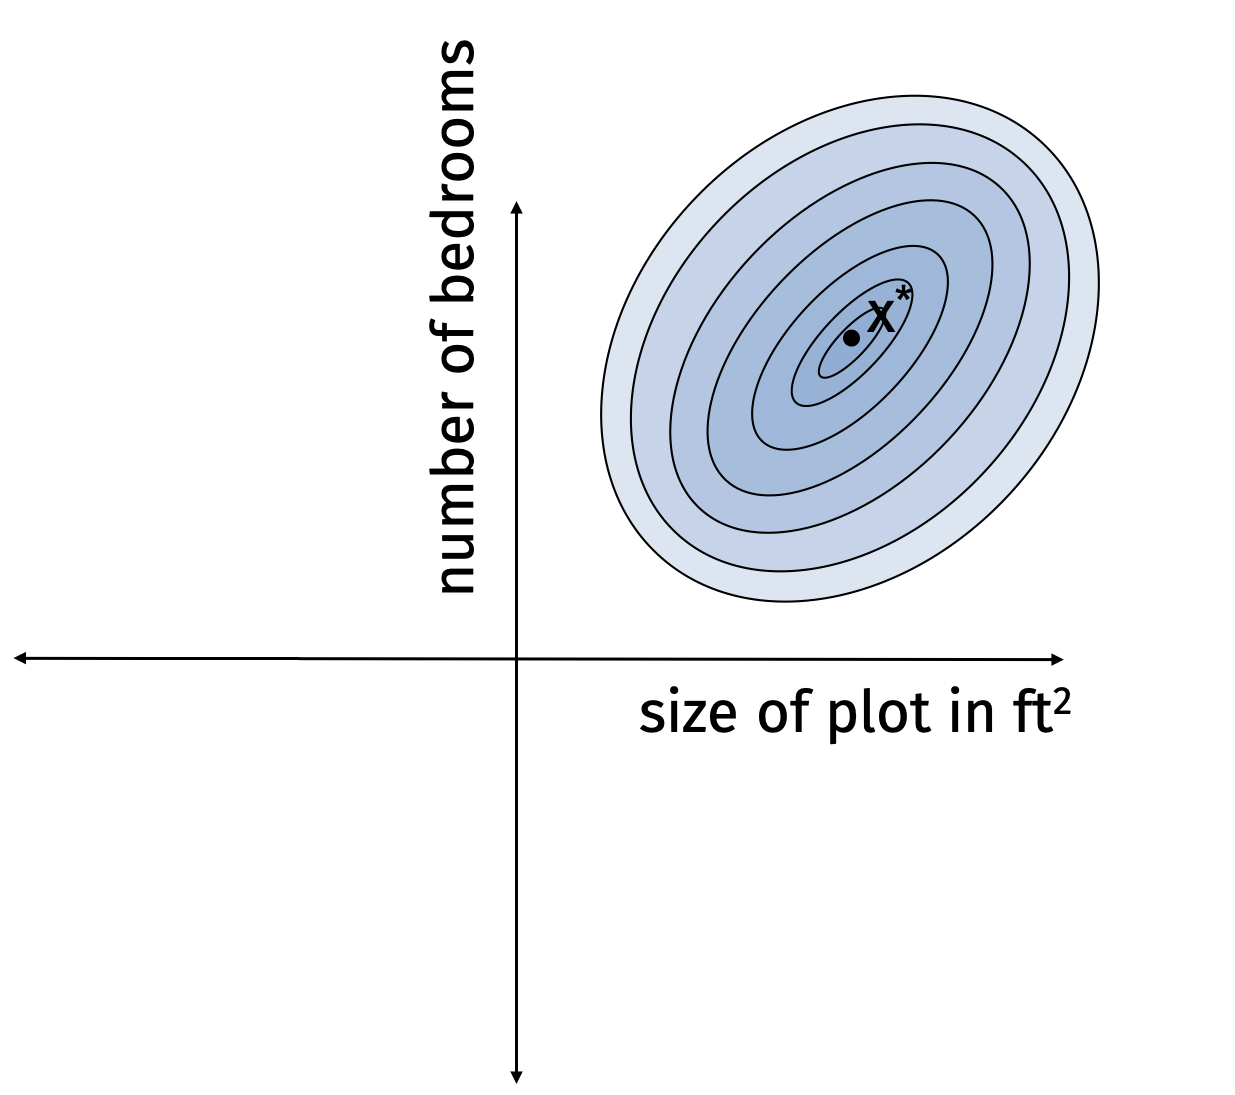
\includegraphics[width=.6\textwidth]{well_conditioned.png}
		\vspace{-.5em}
		
		Feature scaling can have a huge impact on conditioning. 
	\end{center}
\end{frame}

\begin{frame}
	\frametitle{adaptive stepsizes}
	\textbf{Another view}: If $g(\bv{x}) = f(\bv{P}\bv{x})$ then $\nabla g(\bv{x}) = \bv{P}^T\nabla f(\bv{P}\bv{x})$.
	
	$\nabla g(\bv{x})  = \bv{P}\nabla f(\bv{P}\bv{x})$ when $\bv{P}$ is symmetric. 
	
	\vspace{1em}
	\textbf{Gradient descent on $g$:}
	\begin{itemize}
		\item For $t = 1,\ldots, T$,
		\begin{itemize}
			\item $\bv{x}^{(t+1)} = \bv{x}^{(t)} - \eta\bv{P}\left[\nabla f(\bv{P}\bv{x}^{(t)})\right]$
		\end{itemize}
	\end{itemize}
	
	\vspace{1em}
	\textbf{Gradient descent on $g$:}
	\begin{itemize}
		\item For $t = 1,\ldots, T$,
		\begin{itemize}
			\item $\bv{y}^{(t+1)} = \bv{y}^{(t)} - \eta\bv{P}^2\left[\nabla f(\bv{y}^{(t)})\right]$
		\end{itemize}
	\end{itemize}
	\begin{center}
		\alert{When $\bv{P}$ is diagonal, this is just gradient descent with a \emph{different step size for each parameter}!}
	\end{center}
\end{frame}

\begin{frame}
	\frametitle{adaptive stepsizes}
	\textbf{Less clear how to set $\bv{P}$ for general optimization problems where the Hessian is changing, but lots of heuristic algorithms based on this idea:}
	\begin{itemize}
		\item AdaGrad, AdaDelta
		\item RMSprop
		\item Adam optimizer
	\end{itemize}
	\begin{center}
		\vspace{-.5em}
		\alert{(Pretty much all of the most widely used optimization methods for training neural networks.)}
		
		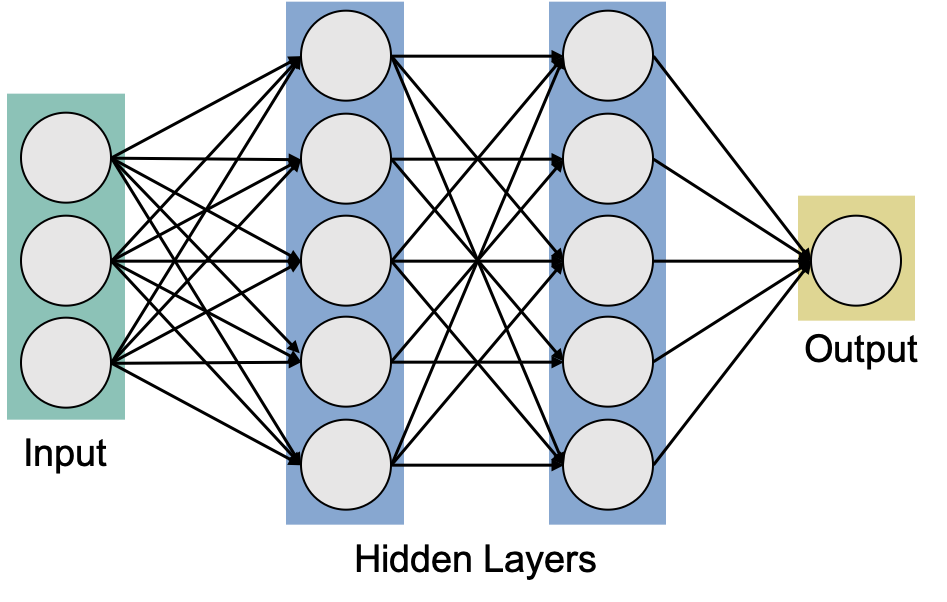
\includegraphics[width=.4\textwidth]{neuralNetwork.png}
	\end{center}
\end{frame}

\begin{frame}[standout]
	\begin{center}
		\large coordinate descent
	\end{center}
\end{frame}

\begin{frame}
	\frametitle{stochastic methods}
	\textbf{Main idea:} Trade slower convergence (more iterations) for cheaper iterations. 
	\vspace{2em}
	
	\textbf{Stochastic Gradient Descent:}
	When $f(\bv{x}) = \sum_{i=1}^n f_i(\bv{x})$, approximate $\nabla f(\bv{x})$ with $\nabla f_i(\bv{x})$ for randomly chosen $i$. 
\end{frame}

\begin{frame}
	\frametitle{stochastic methods}
	\textbf{Main idea:} Trade slower convergence (more iterations) for cheaper iterations. 
	\vspace{2em}
	
	\textbf{Stochastic \alert{Coordinate Descent}:}
	Only compute a \emph{single random entry} of $\nabla f(\bv{x})$ on each iteration:
	\begin{align*}
	\nabla f(\bv{x}) &= 
	\begin{bmatrix}
	\frac{\partial f}{\partial x_1}(\bv{x}) \\ \frac{\partial f}{\partial x_2}(\bv{x}) \\ \vdots \\ \frac{\partial f}{\partial x_d}(\bv{x})  
	\end{bmatrix} & 	\nabla_i f(\bv{x}) &= 
	\begin{bmatrix}
	0\\ \frac{\partial f}{\partial x_i}(\bv{x}) \\ \vdots \\ 0
	\end{bmatrix} 
	\end{align*}
	
\textbf{Update:} $\bv{x}^{(t+1)}\leftarrow \bv{x}^{(t)} - \eta \nabla_i f(\bv{x}^{(t)})$.
\end{frame}

\begin{frame}[t]
	\frametitle{coordinate descent}
	When $\bv{x}$ has $d$ parameters, computing $\nabla_i f(\bv{x})$ \emph{sometimes} costs just a $1/d$ fraction of what it costs to compute $\nabla f(\bv{x})$ 
	
	\vspace{1em}
	\textbf{Example:} $f(\bv{x}) = \|\bv{A}\bv{x} - \bv{b}\|_2^2$ for $\bv{A} \in \R^{n\times d}, \bv{x} \in \R^{d}, \bv{b} \in \R^n$. 
	\begin{itemize}
		\item $\nabla f(\bv{x}) = 2\bv{A}^T\bv{A}\bv{x} - 2\bv{A}^T\bv{b}$.
		\item $\nabla_i f(\bv{x}) = 2\left[\bv{A}^T\bv{A}\bv{x}\right]_i - 2\left[\bv{A}^T\bv{b}\right]_i$.
	\end{itemize}

Computing full gradient takes $O(nd)$ time. Can we do better here?
\end{frame}

\begin{frame}[t]
	\frametitle{coordinate descent}
	When $\bv{x}$ has $d$ parameters, computing $\nabla_i f(\bv{x})$ \emph{sometimes} costs just a $1/d$ fraction of what it costs to compute $\nabla f(\bv{x})$ 
	
	\vspace{1em}
	\textbf{Example:} $f(\bv{x}) = \|\bv{A}\bv{x} - \bv{b}\|_2^2$ for $\bv{A} \in \R^{n\times d}, \bv{x} \in \R^{d}, \bv{b} \in \R^n$. 
	\begin{itemize}
		\item $\nabla f(\bv{x}) = 2\bv{A}^T\bv{A}\bv{x} - 2\bv{A}^T\bv{b}$.
		\item $\nabla_i f(\bv{x}) = 2\left[\bv{A}^T\bv{A}\bv{x}\right]_i - 2\left[\bv{A}^T\bv{b}\right]_i$.
	\end{itemize}
	
	\vspace{2em}
	\begin{itemize}
		\item $\bv{A}\bv{x}^{(t+1)} = \bv{A}\left(\bv{x}^{(t)} + c\cdot \bv{e}_i\right)$ \hspace{4em} \alert{$O(n)$ time}
		\item $2\left[\bv{A}^T \left(\bv{A}\bv{x}^{(t+1)} - \bv{b}\right)\right]_i$ \hspace{6em} \alert{$O(n)$ time}
	\end{itemize}
\end{frame}

\begin{frame}[t]
	\frametitle{stochastic coordinate descent}	
	\textbf{Stochastic Coordinate Descent:}
	\begin{itemize}
		\item Choose number of steps $T$ and step size $\eta$.
		\item For $t = 1,\ldots, T$:
		\begin{itemize}
			\item Pick random $j \in 1, \ldots, d$ uniformly at random.
			\item $\bv{x}^{(t+1)} = \bv{x}^{(t)} - \eta \nabla_{j} f(\bv{x}^{(i)})$
		\end{itemize}
		\item Return $\hat{\bv{x}} = \frac{1}{T}\sum_{t=1}^T \bv{x}^{(t)}$.
	\end{itemize}
\end{frame}

\begin{frame}[t]
	\frametitle{stochastic coordinate descent}
	\begin{theorem}[Stochastic Coordinate Descent convergence]
		Given a $G$-Lipschitz function $f$ with minimizer $\bv{x}^*$ and initial point $\bv{x}^{(1)} $ with $\|\bv{x}^{(1)} - \bv{x}^*\|_2 \leq R$, SCD with step size $\eta = \frac{1}{Rd}$ satisfies the guarantee:
		\begin{align*}
		\E[f(\hat{\bv{x}}) - f({\bv{x}^*})] \leq \frac{2GR}{\sqrt{T/d}}
		\end{align*}
	\end{theorem}
\end{frame}

\begin{frame}[t]
	\frametitle{importance sampling}
	Often it doesn't make sense to sample $i$ uniformly at random:
	\begin{align*}
	\bv{A} &= \begin{bmatrix} 
	0 & 0 & 1 & 0 & 0 & 0 \\
	0 & 0 & 2 & 0 & 0 & 0 \\
	0 & 0 & -1 & 0 & 0 & 0 \\
	0 & 0 & -.5 & 0 & 0 & 0 \\
	0 & 0 & 3 & 0 & 0 & 0 \\
	0 & 0 & -2 & 0 & 0 & 0 
	\end{bmatrix} & 
	\bv{b} &=\begin{bmatrix} 
	 10  \\
	 42 \\
	-11  \\
	 -51 \\
	34\\
	-22 
	\end{bmatrix} 
	\end{align*}
	Select indices $i$ proportional to $\|\bv{a}_i\|_2^2$:
	\begin{align*}
		\Pr[\text{select index $i$ to update}] = \frac{\|\bv{a}_i\|_2^2}{\sum_{j=1}^d \|\bv{a}_j\|_2^2} = \frac{\|\bv{a}_i\|_2^2}{\|\bv{A}\|_F^2} 
	\end{align*}
	\begin{center}
		\alert{\textbf{Let's analyze this approach.}}
	\end{center}
\end{frame}

\begin{frame}[t]
	\frametitle{stochastic coordinate descent}
	Specialization of SCD to $\|\bv{A}\bv{x} - \bv{b}\|_2^2$:
	\vspace{1em}

	\textbf{Randomized Coordinate Descent (Strohmer, Vershynin 2007 / Leventhal, Lewis 2018)}
\begin{itemize}
\item For iterate $\bv{x}^{(t)}$, let $\bv{r}^{(t)}$ be the \emph{residual}:
\begin{align*}
\bv{r}^{(t)} = \bv{A}\bv{x}^{(t)} - \bv{b}
\end{align*}
\item $\bv{x}^{(t+1)} = \bv{x}^{(t)} - c\bv{e}_j$.
\item $\bv{r}^{(t+1)} = \bv{r}^{(t)} - c\bv{a}_j$. Here $\bv{a}_j$ is the $i^\text{th}$ column of $\bv{A}$. 
\end{itemize}

 Typically $c$ depends on fixed learning rate. Here we will choose it \emph{optimally} -- similar idea to gradient descent with \emph{line search}.
\end{frame}

\begin{frame}[t]
	\frametitle{stochastic coordinate descent}
	\begin{center}
		What choice for $c$ minimizes $\|\bv{r}^{(t+1)}\|_2^2$?
	\end{center}

\begin{itemize}
	\item $\|\bv{r}^{(t+1)}\|_2^2 = \|\bv{r}^{(t)} - c\bv{a}_j\|_2^2$
	\item Requires \emph{projecting} $\bv{r}^{(t)}$ onto perpendicular of $\bv{a}_j$.
\end{itemize}
\vspace{-1em}
\begin{center}
	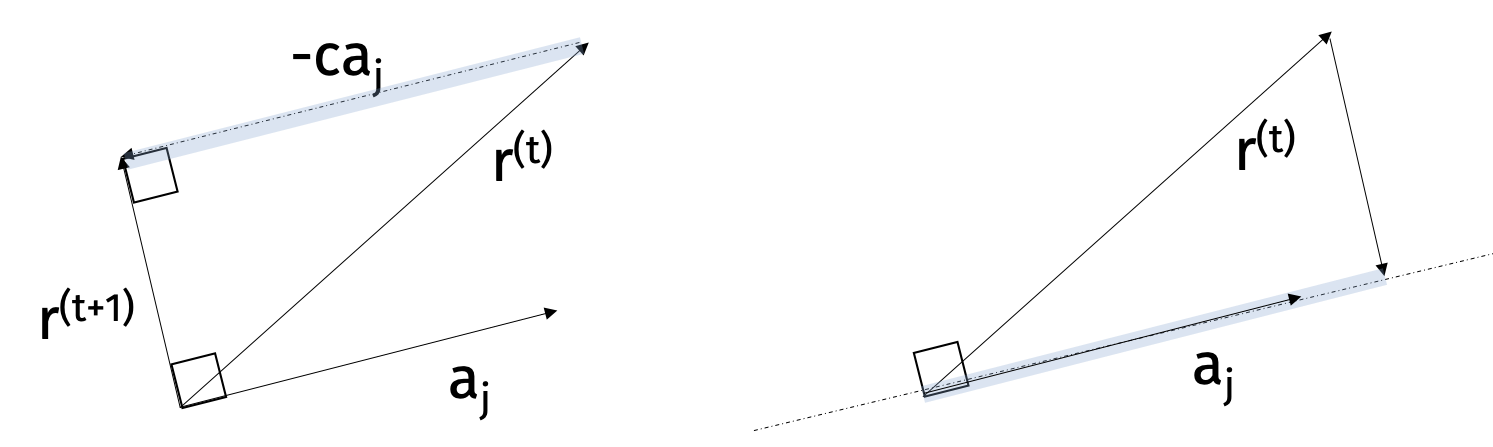
\includegraphics[width=.8\textwidth]{projection.png}
\end{center}
	\begin{itemize}
		\item $c = \frac{\bv{a}_j^T\bv{r}^{(t)}}{\|\bv{a}_j\|_2^2}$
	\end{itemize}

Note that $\|\bv{r}^{(t+1)}\|_2^2 = \|\bv{r}^{(t)}\|_2^2 - \|c\bv{a}_j\|_2^2 = \alert{\|\bv{r}^{(t)}\|_2^2 - \frac{(\bv{a}_j^T\bv{r}^{(t)})^2}{\|\bv{a}_j\|_2^2}}$
\end{frame}


\begin{frame}[t]
	\frametitle{stochastic coordinate descent}
	Specialization of SCD to $\|\bv{A}\bv{x} - \bv{b}\|_2^2$:
	\vspace{1em}
	
	\textbf{Randomized Coordinate Descent}
	\begin{itemize}
		\item Choose number of steps $T$. 
		\item Let $\bv{x}^{(1)} = \bv{0}$ and  $\bv{r}^{(1)} = \bv{b}$.
		\item For $t = 1,\ldots, T$:
		\begin{itemize}
			\item Pick random $j \in 1, \ldots, d$. Index $j$ is selected with probability proportional to $\|\bv{a}_j\|_2^2/\|\bv{A}\|_F^2$.
			\item Set $c = \bv{a}_j^T\bv{r}^{(t)}/\|\bv{a}_j\|_2^2$
			\item $\bv{x}^{(t+1)} = \bv{x}^{(t)} - c \bv{e}_j$
			\item $\bv{r}^{(t+1)} = \bv{r}^{(t)} - c \bv{a}_j$
		\end{itemize}
		\item Return ${\bv{x}^{(T)}}$.
	\end{itemize}
\end{frame}

\begin{frame}[t]
	\frametitle{convergence}
	\begin{claim}
		\begin{align*}
			\E \|\bv{r}^{(t+1)}\|_2^2 = \|\bv{r}^{(t)}\|_2^2 - \frac{1}{\|\bv{A}\|_F^2} \|\bv{A}^T\bv{r}^{(t)}\|_2^2
		\end{align*}
	\end{claim}
\end{frame}

\begin{frame}[t]
	\frametitle{convergence}
	Any residual $\bv{r}$ can be written as $\bv{r} = \bv{r}^* + \bar{\bv{r}}$ where $\bv{r}^*  = \bv{A}\bv{x}^* - \bv{b}$ and  $\bar{\bv{r}} = \bv{A}(\bv{x}^{t} - \bv{x}^*)$. Note that $\bv{A}^T\bv{r}^* = 0$ and $\bar{\bv{r}} \perp \bv{r}^*$.
	\begin{claim}
		\begin{align*}
		\E \|\bar{\bv{r}}^{(t+1)}\|_2^2 
		& \leq \|\bar{\bv{r}}^{(t)}\|_2^2 - \frac{\lmin(\bv{A}^T\bv{A})}{\|\bv{A}\|_F^2} 
		\end{align*}
	\end{claim}

		\begin{align*}
		\E \|\bar{\bv{r}}^{(t+1)}\|_2^2 + \|\bv{r}^*\|_2^2 \leq \|\bar{\bv{r}}^{(t)}\|_2^2 + \|\bv{r}^*\|_2^2 - \frac{1}{\|\bv{A}\|_F^2} \|\bv{A}^T\bar{\bv{r}}^{(t)}\|_2^2  \|\bar{\bv{r}}^{(t)}\|_2^2
		\end{align*}
	
	\textbf{Exercise:} Because $\bar{\bv{r}}$ is in the column span of $\bv{A}$,
		\begin{align*}
		 \|\bv{A}^T\bar{\bv{r}}^{(t)}\|_2^2 \geq \lmin(\bv{A}^T\bv{A})\|\bar{\bv{r}}^{(t)}\|_2^2
		\end{align*}
\end{frame}

\begin{frame}[t]
	\frametitle{convergence}
		\begin{theorem}[Randomized Coordinate Descent convergence]
			After $T$ steps of RCD with importance sampling run on $f(\bv{x}) = \|\bv{A}\bv{x} - \bv{b}\|_2^2$, we have:
			\begin{align*}
			\E[f(\bv{x}^{(t)}) - f(\bv{x}^*)] \leq\left(1 - \frac{\lmin(\bv{A}^T\bv{A})}{\|\bv{A}\|_F^2}\right)^t [f(\bv{x}^{(0)}) - f(\bv{x}^*)] 
			\end{align*}
		\end{theorem}
		\textbf{Corollary:} After $T = O(\frac{\|\bv{A}\|_F^2}{\lmin(\bv{A}^T\bv{A})}\log\frac{1}{\epsilon})$ we obtain error $\epsilon \|\bv{b}\|_2^2$.
		
		\vspace{5em}
		\alert{Is this more or less iterations than the $T = O(\frac{\lmax(\bv{A}^T\bv{A})}{\lmin(\bv{A}^T\bv{A})}\log\frac{1}{\epsilon})$ required for gradient descent to converge?}
\end{frame}

\begin{frame}[t]
	\frametitle{comparison}
	\textbf{Recall useful linear algebraic fact:}
	\begin{align*}
	\|\bv{A}\|_F^2 = \tr(\bv{A}^T\bv{A}) = \sum_{i=1}^d \lambda_i(\bv{A}^T\bv{A})
	\end{align*}
	
	\begin{align*}
	\lmax(\bv{A}^T\bv{A}) \leq \|\bv{A}\|_F^2 \leq d\cdot \lmax(\bv{A}^T\bv{A})
	\end{align*}
	
	\vspace{1em}
	\textbf{For solving $\|\bv{A}\bv{x} - \bv{b}\|_2^2$},
	\begin{align*}
	\text{($\#$ GD Iterations)}\leq \text{($\#$ RCD Iterations)} \leq d\cdot \text{($\#$ GD Iterations)}
	\end{align*}
	\begin{center}
		\alert{\textbf{But RCD iterations are cheaper by a factor of $d$.}}
	\end{center}
\end{frame}

\begin{frame}[t]
	\frametitle{comparison}
	\textbf{When does $\|\bv{A}\|_F^2 = \tr(\bv{A}^T\bv{A})  = \alert{d}\cdot \lmax(\bv{A}^T\bv{A})$?}
	\vspace{8em}
	
		\textbf{When does $\|\bv{A}\|_F^2 = \tr(\bv{A}^T\bv{A})  = \alert{1}\cdot \lmax(\bv{A}^T\bv{A})$?}
	
\end{frame}

\begin{frame}
	\frametitle{comparison}
	\begin{center}
		Roughly:
	\end{center}
	\textbf{Stochastic Gradient Descent} performs well when \emph{data points} (rows) are repetitive. 
	
	\vspace{1em}
	\textbf{Stochastic Coordinate Descent} performs well when \emph{data features} (columns) are repetitive. 
\end{frame}

\begin{frame}[standout]
	\begin{center}
		\large non-convex optimization
	\end{center}
\end{frame}


\begin{frame}[t]
	\frametitle{stationary points}
	We understand much less about optimizing non-convex functions in comparison to convex functions, but not nothing. In many cases, we're still figuring out the right questions to ask
	\begin{definition}[Stationary point]
		For a differentiable function $f$, a \emph{stationary point} is any $\bv{x}$ with: 
		\begin{align*}
		\nabla f(\bv{x}) = \bv{0}
		\end{align*}
	\end{definition}
	\begin{center}
		local/global minima - local/global maxima - saddle points
	\end{center}
\end{frame}

\begin{frame}[t]
	\frametitle{stationary points}
	\textbf{Reasonable goal:} Find an \emph{approximate stationary point} $\hat{\bv{x}}$ with
	\begin{align*}
		\|\nabla f(\hat{\bv{x}})\|_2^2 \leq \epsilon.
	\end{align*}
\end{frame}

\begin{frame}[t]
	\frametitle{smoothness for non-convex funtions}
	\begin{definition}
		A differentiable (potentially non-convex) function $f$ is $\beta$ smooth if \emph{for all} $\bv{x}, \bv{y}$, 
		\begin{align*}
		\|\nabla f(\bv{x}) - \nabla f(\bv{y})\|_2 \leq \beta \|\bv{x} - \bv{y}\|_2
		\end{align*}
	\end{definition}
	\textbf{Corollary:} For all $\bv{x}, \bv{y}$
	\begin{align*}
	\left | \nabla f(\bv{x})^T(\bv{x} - \bv{y}) - [f(\bv{x}) - f(\bv{y})] \right| \leq \frac{\beta}{2} \|\bv{x} - \bv{y}\|_2^2.
	\end{align*}
\end{frame}


\begin{frame}[t]
	\frametitle{gradient descent finds approximate stationary points}
	\begin{theorem}
		If GD is run with step size $\eta = \frac{1}{\beta}$ on a differentiable function $f$ with global minimum $\bv{x}^*$ then after $T = O(\frac{\beta [f(\bv{x}^{(1)}) - f(\bv{x}^*)]}{\epsilon})$ we will find an $\epsilon$-approximate stationary point $\hat{\bv{x}}$.
	\end{theorem}
\begin{itemize}
	\item  $ \nabla f(\bv{x}^{(t)})^T(\bv{x}^{(t)} - \bv{x}^{(t+1)}) - f(\bv{x}^{(t)}) + f(\bv{x}^{(t+1)}) \leq \frac{\beta}{2}\|\bv{x}^{(t)} - \bv{x}^{(t+1)}\|_2^2.$
	\item $f(\bv{x}^{(t+1])}) - f(\bv{x}^{(t)}) \leq \frac{\beta}{2}\eta^2\|\nabla f(\bv{x}^{(t)})\|_2^2 - \eta \|\nabla f(\bv{x}^{(t)})\|_2^2$ 
	\item $f(\bv{x}^{(t+1])}) - f(\bv{x}^{(t)}) \leq \frac{-\eta}{2}\|\nabla f(\bv{x}^{(t)})\|_2^2$
	\item $\frac{1}{T}\sum_{t=1}^T \frac{\eta}{2}\|f(\bv{x}^{(t)})\|_2^2 \leq \frac{1}{T}\sum_{t=1}^T f(\bv{x}^{(t)}) - f(\bv{x}^{(t+1)})$
	\item $\frac{\eta}{2} \min_t \|f(\bv{x}^{(t)})\|_2^2 \leq \frac{1}{T}\left[f(\bv{x})^{(1)} - f(\bv{x})^{(T)})\right]$
\end{itemize}
	
\end{frame}

\begin{frame}[t]
	\frametitle{questions in non-convex optimization}
	\textbf{If GD can find a stationary point, are there algorithms which find a stationary point faster using preconditioning, acceleration, stocastic methods, etc.?}
\end{frame}

\begin{frame}[t]
	\frametitle{questions in non-convex optimization}
	\textbf{What if my function only has global minima and stationary points?}
	Randomized methods (SGD, perturbed gradient methods, etc.) can ``escape'' stationary points under some minor assumptions.
	\vspace{1em}
	
	
	\textbf{Example:} $\min_{\bv{x}} \frac{-\bv{x}^T\bv{A}^T\bv{A}\bv{x}}{\bv{x}^T\bv{x}}$
	\begin{itemize}
		\item \textbf{Global minimum}: Top eigenvector of $\bv{A}^T\bv{A}$ (i.e., top principal component of $\bv{A}$).
		\item \textbf{Stationary points:} All other eigenvectors of $\bv{A}$. 
	\end{itemize}
\begin{center}
	\alert{Useful for lots of other matrix factorization problems beyond vanilla PCA.}
\end{center}
\end{frame}


\end{document} 








